\section{Umsetzung}
\subsection{Entwicklung}
Die Anwendung wurde mit Java 7 entwickelt. Als Entwicklungsumgebung wurde Eclipse in Verbindung mit Maven eingesetzt. 

\subsection{Verwendete Bibliotheken}
Im Rahmen der Entwicklung wurden diverse OpenSource-Bibliotheken eingeführt, um die Entwicklung zu beschleunigen und die Qualität der Software zu steigern. Im folgenden werden die verwendeten Bibliotheken beschrieben:
\begin{description}
 \item[Apache Commons Math] (Version 3.2, Apache License 2.0) \cite{apache:CommonsMath} Stellt mathematische Funktionen zur Verfügung. Wird unteranderem für die Berechnung der Entfernungen verwendet.
 \item[Apache Commons Lang] (Version 3.3.1, Apache License 2.0) \cite{apache:CommonsLang} Stellt allgemeine Java-Funktionen zur Verfügung.
 \item[Apache Commons Collections] (Version 4.0, Apache License 2.0) \cite{apache:CommonsCollection} Erweitert das Java-Collec\-tions-Framework. 
 \item[Joda-Time] (Version 2.3, Apache License 2.0) \cite{joda:jodatime} Bietet eine umfassende Bibliothek zur Zeitmessung.
 \item[JUnit] (Version 4.11, Eclipse Public License) \cite{junit:junit} JUnit ist die Standard-Bibliothek für Unit-Tests unter Java. 
 \item[Hamcrest] (Version 1.3, BSD 3-Clause) \cite{hamcrest:hamcrest} Mit Hamcrest ist es möglich bei Tests "`sprechendere"' Ausdrücke zu formulieren.
 \item[EasyMock] (Version 3.2, Apache License 2.0) \cite{easymock:easymock} EasyMock ermöglicht ein einfaches Erstellen von Mock-Objekten für den Unit-Test.
 \item[Simple Logging Facade for Java (SL4J)] (Version 1.7.6, MIT license) \cite{qos:slfj} SLF4J ist eine Log\-ging-Schnittstelle und wird zur Ausgabe auf der Konsole verwendet.
 \item[Logback] (Version 1.1.1, Eclipse Public License v1.0 und LGPL 2.1) \cite{qos:logback} Wird als Implementierung für SLF4J eingesetzt.
 \item[Google Guave] (Version 17.0, Apache License 2.0) \cite{google:guave} Guave ist eine Sammlung von Softwarebibliotheken. Es wird ausschließlich der EventBus für die Kommunikation zwischen den Softwarekomponenten verwendet.
 \item[JFreeChart] (Version 1.0.17, LPGL) \cite{ObjectRefineryLimited:JFreeChart} JFreeChart wird zur Darstellung der Graphen verwendet.
\end{description}

\newpage
\subsection{Populationssortierung}
Das Sortieren der Population geschieht mit Hilfe des \java{PlanComparator}s (\Fref{fig:PlanComparator}). Dieser sortiert zuerst mit Hilfe des \java{Validator}s die gültigen und ungültigen Individuen und im Anschluss die beiden Gruppen nach ihrem Fitnesswert. Somit stehen gültige Individuen immer über ungültigen Individuen.
\myfigure[width=0.95\textwidth]{PlanComparator}{../src/main/java/de/hsbremen/kss/genetic/PlanComparator.png}{Sortierung der Population}

\subsection{Validation}
Es wurden zwei Validatoren (siehe \Fref{fig:Validator}) implementiert. Der \java{FullValidator} prüft alle Restriktionen (vgl. \Fref{sec:Restriktionen}). Er wird am Ende der Optimierung verwendet um das beste Ergebnis zu überprüfen. Für das Sortieren der Population wird hingegen der \java{RightOrderValidatorImpl} verwendet. Er führt eine schwächere Prüfung durch und ignoriert unteranderem die Verletzungen von Zeitfenstern.
\myfigure[width=0.5\textwidth]{Validator}{../src/main/java/de/hsbremen/kss/validate/Validator.png}{Implementierte Validatoren}

\newpage
\subsection{Fitnesstest}
\Fref{fig:Fitness} zeigt die implementierten Fitness Tests. Sie lassen sich dynamisch zusammenschalten und konfigurieren.
\myfigure[width=0.8\textwidth]{Fitness}{../src/main/java/de/hsbremen/kss/genetic/fitness/FitnessTest.png}{Implementierte Fitness Tests}

\subsection{Selektion}
Es wurden drei unterschiedliche Selektionsverfahren entwickelt (siehe \Fref{fig:Selektion}). Die \java{RandomSelektion} wählt zufällig ein Individuum aus der Population aus. Die \java{OnyTheBest\-Selection} wählt aus den Besten (konfigurierbar) zufällig ein Individuum aus. Die \java{Linear\-Distribution\-Selection} wählt die Individuen mit einem höheren Rang mit einer höheren Wahrscheinlichkeit aus. Die \Fref{fig:SelektionGraph} verdeutlicht die unterschiedlichen Selektionsarten anhand von drei Graphen.
\myfigure[width=0.8\textwidth]{Selektion}{../src/main/java/de/hsbremen/kss/genetic/selection/Selektion.png}{Implementierte Selektionen}

\begin{figure}
	\centering
      \subfigure[LinearSelectionImpl]{
	\label{fig:SelektionLinear}
	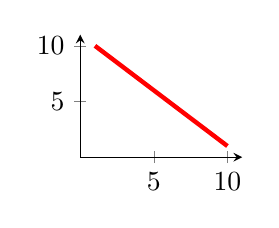
\begin{tikzpicture}
		\begin{axis}[
		xmin=0, xmax=11,
		ymin=0, ymax=11,
		axis lines=center,
		axis on top=true,
		domain=1:10,
		width=0.3\textwidth,
		]

		\addplot [mark=none,draw=red,ultra thick] {11-x};
		\end{axis}
		\end{tikzpicture}

      }
      \hspace{0.2cm}
      \subfigure[RandomSelektion]{
	\label{fig:SelektionRandom}
		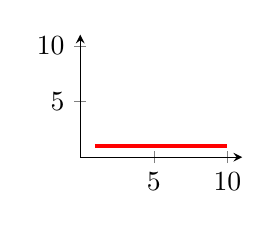
\begin{tikzpicture}
		\begin{axis}[
		xmin=0, xmax=11,
		ymin=0, ymax=11,
		axis lines=center,
		axis on top=true,
		domain=1:10,
		width=0.3\textwidth,
		]

		\addplot [mark=none,draw=red,ultra thick] {1};
		\end{axis}
		\end{tikzpicture}
      }
      \hspace{0.2cm}
      \subfigure[OnlyTheBestSelection]{
	\label{fig:SelektionOnlyBest}
	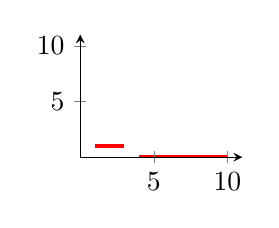
\begin{tikzpicture}
	\begin{axis}[
	xmin=0, xmax=11,
	ymin=0, ymax=11,
	axis lines=center,
	axis on top=true,
	width=0.3\textwidth,
	]

	\addplot [mark=none,draw=red,ultra thick,domain=1:3] {1};
	\addplot [mark=none,draw=red,ultra thick,domain=4:10] {0};
	\end{axis}
	\end{tikzpicture}
      }
      \caption{Selektion bei einer Populationsgröße von 10 Individuen (X: Individuenrang, Y: Wahrscheinlichkeit)}
      \label{fig:SelektionGraph}
\end{figure}

\newpage
\subsection{Crossover}
Als wurde Crossover (siehe \Fref{fig:Crossover}) wurde nur der Crossover mit Controlstring implementiert (vgl. \Fref{sec:CrossoverControlString}).
\myfigure[width=0.7\textwidth]{Crossover}{../src/main/java/de/hsbremen/kss/genetic/crossover/Crossover.png}{Implementierter Crossover}

\subsection{Mutation}
Im Klassendiagramm (\Fref{fig:Mutation}) sind alle implementierten Mutationen dargestellt. Instanzen dieser Mutationen werden dem genetischen Algorithmus übergeben. Dieser wählt dabei zufällig eine Mutation aus und wendet sie auf ein Individuum an. Es können auch "`null"'-Mutationen übergeben werden. Dies bedeutet, dass das Individuum nicht mutiert wird. Hierüber lässt sich die Mutationsrate steuern.

Die Mutationen sind so implementiert, dass sie möglichst nur gültige Lösungen liefern (Kein Abladen vor dem Aufladen; nur Produkte aufladen, die auch mit dem Fahrzeug transportiert werden können). 
\myfigure[width=0.95\textwidth]{Mutation}{../src/main/java/de/hsbremen/kss/genetic/mutation/Mutation.png}{Implementierte Mutationsalgorithmen}



\newpage
\subsection{Grafische Oberfläche}
\label{sec:GrafischeOberflaeche}
Die drei folgenden Abbildungen zeigen die grafische Oberfläche. Sie wird beider jeder Iteration aktualisiert und zeigt somit immer den aktuellen Stand.

\Fref{fig:Map} zeigt eine Deutschlandkarte auf welcher das beste Individuum abgebildet wird. Die unterschiedlichen Farben symbolisieren unterschiedliche Touren.

\Fref{fig:FitnessDistribution} zeigt die relativen Aufbau des Fitnesswertes. Aus diesem Graphen lässt sich entnehmen, ob es noch Verletzungen von Restriktionen gibt und was der genetische Algorithmus zur Zeit optimiert.

\Fref{fig:FitnessLengthGraph} zeigt die Entwicklung des Fitness Wertes und der Gesamtstreckenlänge. Der Fitness Wert sinkt stetig. Die Streckenlänge kann sich auch wieder verschlechtern, wenn hierdurch andere Verletzung vermieden werden.

\myfigure[scale=0.6]{Map}{Map.png}{Das beste Ergebnis wird auf einer Deutschlandkarte dargestellt}
\myfigure[scale=0.6]{FitnessDistribution}{FitnessDistribution.png}{Verteilung des Fitnesswertes}
\myfigure[scale=0.6]{FitnessLengthGraph}{FitnessLengthGraph.png}{Fitness Wert und Länge des besten und schlechtesten Individuum + Durchschnitt über die gesamt Population}


